\section{Additional Generality Results}
\label{app:generality}

We evaluate generality along three deployment dimensions: cluster resource
distribution, function-set size, and function-popularity distribution. We report
CPU utilization and task throughput as representative metrics. All improvements
at 100\% offered load are relative to the best-performing baseline for the
corresponding metric. Because Golgi and Golgi-NoCC exhibit only minor differences,
we report only Golgi in these experiments.

\begin{figure}[t]
    \centering
    
\includegraphics[width=0.86\linewidth]{figures/fig_gen_resource_dist_legend.pdf}\\[-10pt]
    \subfloat[]{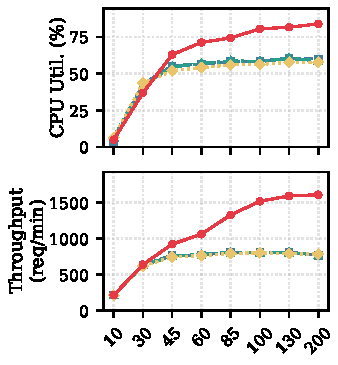
\includegraphics[width=0.552\linewidth]{figures/fig_gen_simple_compact.pdf}%
        \label{fig:gen_simple}}
    \hspace{-0.02\linewidth}
    \subfloat[]{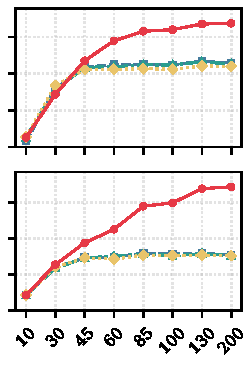
\includegraphics[width=0.410\linewidth]{figures/fig_gen_zipf_compact.pdf}%
        \label{fig:gen_zipf}}
    \\[-16pt]\makebox[\linewidth][c]{\footnotesize \qquad Load (\% of cluster capacity)}
    \caption{Performance under different cluster resource distributions. Each
    subfigure shows CPU utilization (top) and task throughput (bottom):
    (a) uniform and (b) Zipf.}
    \label{fig:gen_resource_dist}
\end{figure}

\textbf{Resource distributions.}
Figure~\ref{fig:gen_resource_dist} compares uniform and Zipf-distributed resource
availability. The uniform setting exposes 75\% of each server's capacity, whereas
the Zipf setting uses eight resource tiers with $\alpha=0.8$. At 100\% load,
COSMOS improves CPU utilization by 37.63\% and 43.04\%, and throughput by 87.30\%
and 90.10\%, under the uniform and Zipf settings, respectively. Its advantage
therefore persists under both balanced and highly heterogeneous availability.

\begin{figure}[t]
    \centering
    
\includegraphics[width=0.86\linewidth]{figures/fig_gen_funcnum_legend.pdf}\\[-10pt]
    \subfloat[]{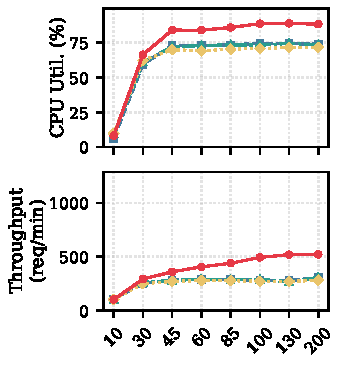
\includegraphics[width=0.552\linewidth]{figures/fig_gen_func5_compact.pdf}%
        \label{fig:gen_func5}}
    \hspace{-0.02\linewidth}
    \subfloat[]{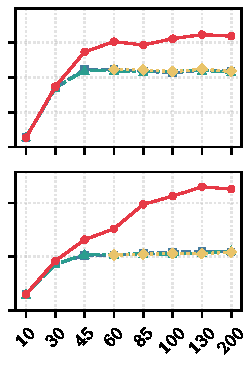
\includegraphics[width=0.410\linewidth]{figures/fig_gen_func20_compact.pdf}%
        \label{fig:gen_func20}}
    \\[-16pt]\makebox[\linewidth][c]{\footnotesize \qquad Load (\% of cluster capacity)}
    \caption{Performance with different numbers of functions. Each subfigure
    shows CPU utilization (top) and task throughput (bottom): (a) five and
    (b) twenty functions.}
    \label{fig:gen_funcnum}
\end{figure}

\textbf{Number of functions.}
We compare the default ten-function workload with two additional settings. The
five-function setting uses video-processing, graph-pagerank, image-recognition,
dna-visualisation, and thumbnailer, doubling each invocation rate to preserve
aggregate load. The twenty-function setting adds a logically distinct replica
of each original function and halves every per-function invocation rate. At
100\% load, COSMOS improves CPU utilization by 19.15\% and 42.73\%, and throughput
by 70.44\% and 94.97\%, with five and twenty functions, respectively. Greater
function diversity provides more opportunity to improve locality and complementary
resource matching.

\begin{figure}[t]
    \centering
    
\includegraphics[width=0.86\linewidth]{figures/fig_gen_workload_legend.pdf}\\[-10pt]
    \subfloat[]{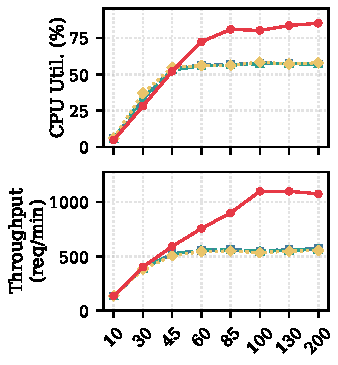
\includegraphics[width=0.552\linewidth]{figures/fig_gen_workload_default_compact.pdf}%
        \label{fig:gen_workload_default}}
    \hspace{-0.02\linewidth}
    \subfloat[]{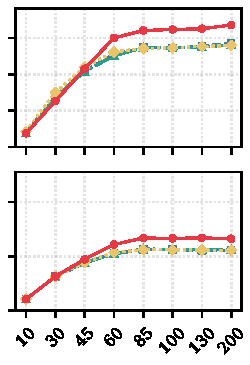
\includegraphics[width=0.410\linewidth]{figures/fig_gen_skewed_compact.pdf}%
        \label{fig:gen_skewed}}
    \\[-16pt]\makebox[\linewidth][c]{\footnotesize \qquad Load (\% of cluster capacity)}
    \caption{Performance under different popularity distributions. Each
    subfigure shows CPU utilization (top) and task throughput (bottom):
    (a) default and (b) 80/20 skewed.}
    \label{fig:gen_workload_dist}
\end{figure}

\textbf{Workload distributions.}
We compare the default workload with an 80/20 popularity skew while preserving
the aggregate invocation rate. In the skewed setting, thumbnailer and
video-processing collectively account for 80\% of invocations. At 100\% load,
COSMOS improves CPU utilization by 37.34\% and throughput by 99.56\% under the
default workload; under the 80/20 workload, the gains are 18.31\% and 18.00\%.
Concentration on two functions naturally improves reuse for all systems and
reduces COSMOS's optimization headroom, but COSMOS retains an advantage.
